\begin{figure}[htbp]
\centering
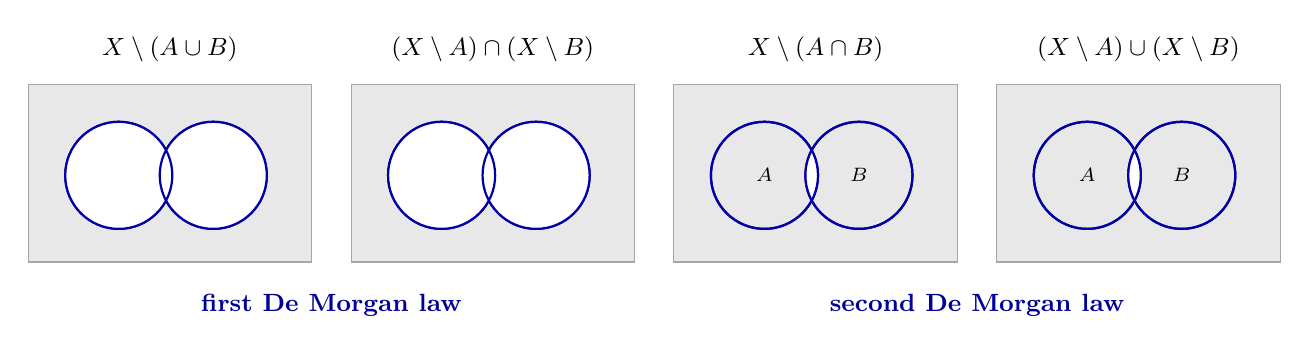
\begin{tikzpicture}[font=\scriptsize]
    \node[font=\small\bfseries] at (1.8,2.7) {$X\setminus(A\cup B)$};
    \node[font=\small\bfseries] at (5.9,2.7) {$(X\setminus A)\cap(X\setminus B)$};
    \node[font=\small\bfseries] at (10.0,2.7) {$X\setminus(A\cap B)$};
    \node[font=\small\bfseries] at (14.1,2.7) {$(X\setminus A)\cup(X\setminus B)$};
    \foreach \shift in {0,4.1,8.2,12.3} {
        \begin{scope}[xshift=\shift cm]
            \fill[gray!18] (0,0) rectangle (3.6,2.25);
            \draw[gray!70] (0,0) rectangle (3.6,2.25);
            \draw[blue!65!black,thick] (1.15,1.1) circle (0.68);
            \draw[blue!65!black,thick] (2.35,1.1) circle (0.68);
            \node at (1.15,1.1) {$A$};
            \node at (2.35,1.1) {$B$};
        \end{scope}
    }
    \begin{scope}[xshift=0cm]
        \fill[white] (1.15,1.1) circle (0.68);
        \fill[white] (2.35,1.1) circle (0.68);
        \draw[blue!65!black,thick] (1.15,1.1) circle (0.68);
        \draw[blue!65!black,thick] (2.35,1.1) circle (0.68);
    \end{scope}
    \begin{scope}[xshift=4.1cm]
        \fill[white] (1.15,1.1) circle (0.68);
        \fill[white] (2.35,1.1) circle (0.68);
        \draw[blue!65!black,thick] (1.15,1.1) circle (0.68);
        \draw[blue!65!black,thick] (2.35,1.1) circle (0.68);
    \end{scope}
    \begin{scope}[xshift=8.2cm]
        \begin{scope}
            \clip (1.15,1.1) circle (0.68);
            \fill[white] (2.35,1.1) circle (0.68);
        \end{scope}
        \draw[blue!65!black,thick] (1.15,1.1) circle (0.68);
        \draw[blue!65!black,thick] (2.35,1.1) circle (0.68);
    \end{scope}
    \begin{scope}[xshift=12.3cm]
        \begin{scope}
            \clip (1.15,1.1) circle (0.68);
            \fill[white] (2.35,1.1) circle (0.68);
        \end{scope}
        \draw[blue!65!black,thick] (1.15,1.1) circle (0.68);
        \draw[blue!65!black,thick] (2.35,1.1) circle (0.68);
    \end{scope}
    \node[font=\small\bfseries,text=blue!60!black] at (3.85,-0.55) {first De Morgan law};
    \node[font=\small\bfseries,text=blue!60!black] at (12.05,-0.55) {second De Morgan law};
\end{tikzpicture}
\caption{The paired shaded regions agree: taking a complement turns a union into an intersection of complements, and turns an intersection into a union of complements.}
\label{fig:demorgan-laws}
\end{figure}